\documentclass{article}
\usepackage[utf8]{inputenc}
\usepackage[russian]{babel}
\usepackage{amsfonts}
\usepackage{amsmath}
\usepackage{natbib}
\usepackage{upquote}
\usepackage{datetime}
\usepackage{multicol}
\usepackage{listings}
\usepackage{graphicx}
\usepackage{enumitem}


\setlength{\voffset}{-2cm}
\setlength{\textheight}{600pt}

\title{Численные методы: Домашняя работа}
\author{Группа 4001BV: Карина Пилюшонока}
\date \today

\begin{document}

\maketitle
\newpage
\tableofcontents
\newpage
\section{Расчет индивидуальных коэффициентов для заданий}
Номер группы: 4001BV \\
Номер в журнале: 16 \\
Год посутпления: 2010 \\
Форма обучения: вечерняя

\begin{displaymath} 
  N_{g} = 3 \cdot (4 + 2) + 0 - 1 = 17
\end{displaymath}

\begin{displaymath}
  N_{s} = 16
\end{displaymath}
\section{Метод исключения Гаусса}

\begin{displaymath}
\left(
  \begin{array}{ccc}
    (N_{g}+4)+5i & -3-4i & 4-4i \\
    -3+2i & 8+(10-N_{s})i & 1+2i \\
    (N_{g}+1)i & N_{s}-10 & N_{s}-N_{g}i
  \end{array}
\right)
=
\left(
  \begin{array}{ccc}
    3+6i\\
    1-(N_{s}-20)i\\
    10i
  \end{array}
\right)
\end{displaymath}
После отброса мнимой части из уравнений получаем следующие коэффициенты для
уравнений:
\begin{displaymath}
\left(
  \begin{array}{ccc}
    21 x_{1} & -3 x_{2} & 4 x_{3} \\
    -3 x_{1} & 8 x_{2} & 1 x_{3} \\
    0 & 6 x_{2} & 16 x_{3}
  \end{array}
\right)
=
\left(
  \begin{array}{ccc}
    3\\
    1\\
    0
  \end{array}
\right)
\end{displaymath}

\subsection{Прямой ход Гаусса}
итерация: 1 

$I * -\frac{a_{21}}{a_{11}} + II$, где 
$I * -\frac{a_{21}}{a_{11}}$ принимает вид $3 - \frac{3}{7} + \frac{4}{7} =
\frac{3}{7}$
\begin{displaymath}
\left(
  \begin{array}{ccc}
    21 x_{1} & -3 x_{2} & 4 x_{3} \\
    0 & 7 \frac{4}{7} x_{2} & 1 \frac{4}{7} x_{3} \\
    0 & 6 x_{2} & 16 x_{3}
  \end{array}
\right)
=
\left(
  \begin{array}{ccc}
    3\\
    1\frac{3}{7}\\
    0
  \end{array}
\right)
\end{displaymath}
итерация: 2

$II * -\frac{a_{32}}{a_{22}} + III$, где 
$II * -\frac{a_{32}}{a_{22}}$ принимает вид $0 - 6 - 1\frac{13}{53} =
-1\frac{7}{53}$
\begin{displaymath}
\left(
  \begin{array}{ccc}
    21 x_{1} & -3 x_{2} & 4 x_{3} \\
    0 & 7 \frac{4}{7} x_{2} & 1 \frac{4}{7} x_{3} \\
    0 & 0 & 14\frac{40}{53} x_{3}
  \end{array}
\right)
=
\left(
  \begin{array}{ccc}
    3\\
    1\frac{3}{7}\\
    -1\frac{7}{53}
  \end{array}
\right)
\end{displaymath}

\subsection{Обратный ход Гаусса}

$x_{3} = -1\frac{7}{53} / 14\frac{40}{53} 
= -\frac{60}{53}/\frac{782}{53} 
= -\frac{60}{782} 
= -\frac{30}{391} \\$
$x_{2} = \frac{1\frac{3}{7} - 1\frac{4}{7} * (-\frac{30}{391})}{7 \frac{4}{7}} 
= (\frac{10}{7} + \frac{330}{2373}) / \frac{53}{7} 
= \frac{3910 + 330}{2737} / \frac{53}{7} 
= \frac{4240 * 7}{2737 * 53} 
= \frac{80}{391}\\$
$x_{1} = \frac{3 - 4*\frac{-30}{391} + 3*\frac{80}{391}}{21}
= (3 + \frac{120}{391} + \frac{240}{391})/21
= 3\frac{360}{391} / 21
= \frac{1533}{391 * 21} 
= \frac{73}{391}$
\begin{displaymath}
\mathbf{X} =
\left( \begin{array}{ccc}
  \frac{73}{391}\\ \\
  \frac{80}{391}\\ \\
  \frac{-30}{391} 
\end{array} \right)
\end{displaymath}

\subsection{Проверка}
yравнение 1:\\
$21 * \frac{73}{391} -3*\frac{80}{391} + 4 * \frac{-30}{391}
= \frac{1533}{391} - \frac{360}{391}
= \frac{1173}{391} 
= 3$
\\\\
yравнение 2:\\
$ -3 * \frac{73}{391} + 8*\frac{80}{391} + 1 *\frac{-30}{391}
= \frac{-219}{391} + \frac{640}{391} - \frac{-30}{391}
= 1$
\\\\
yравнение 3:\\
$0 + 6*\frac{80}{391} + 16 *\frac{-30}{391}
= \frac{480}{391} -\frac{480}{391} 
= 0$

\section{Методы приближения функции. Интерполяция и аппроксимация}

\begin{table}[!h]
  \begin{tabular}{|l|l|l|l|l|}
  \hline
  \bfseries x & -1 & $N_{g}$   & 6 & 10\\
  \hline
  \bfseries y &  1 & $N_{s}-5$ & 8 & -2\\
  \hline
  \end{tabular}
\end{table}
При подстановке $N_{g}$ и $N_{s}$ получим следующий набор узлов:
\begin{table}[!h]
  \begin{tabular}{|l|l|l|l|l|}
  \hline
  \bfseries x & -1 & $17$ & 6 & 10\\
  \hline
  \bfseries y &  1 & $11$ & 8 & -2\\
  \hline
  \end{tabular}
\end{table}
 
\subsection{Полином Лагранжа}
Составляется полином для заданных узлов.\\
\begin{math}
  \frac{(x-17)(x-6)(x-10)}{(-1-17)(-1-6)(-1-10)} \cdot 1 +
  \frac{(x+1)(x-6)(x-10)}{(17+1)(17-6)(17-10)} \cdot 11 +
  \frac{(x+1)(x-17)(x-10)}{(6+1)(6-17)(6-10)} \cdot 8 + 
  \frac{(x+1)(x-17)(x-6)}{(10+1)(10-17)(10-6)} \cdot (-2)
\end{math}\\

Далее, раскрываются скобки, а также в 1ой и 4ой дроби меняем знак изза
полученных знаков в знаменателе. \\
\begin{math} 
  \frac{-x^3 + 33x^2 - 332x + 1020}{1386} +
  \frac{11x^3 - 165x^2 + 484x + 660}{1386} + 
  \frac{8x^3 -208x^2 + 1144x + 1360}{308} + 
  \frac{2x^3 - 44x^2 + 158x + 204}{308}
\end{math}\\

Далее складываем попарно дроби (1+2 и 3+4).\\
\begin{math} 
  \frac{-x^3 + 33x^2 - 332x + 1020 + 11x^3 - 165x^2 + 484x + 660}{1386} +
  \frac{8x^3 -208x^2 + 1144x + 1360 + 2x^3 - 44x^2 + 158x + 204}{308} =
  \frac{10x^3 + -132x^2 + 152x + 1680 }{1386} +
  \frac{10x^3 -252x^2 + 1302x + 1564}{308} =
  \frac{10x^3 + -132x^2 + 152x + 1680 }{1386} +
  \frac{5x^3 -126x^2 + 651x + 782}{154}    
\end{math}\\

Приведение дроби к общему знаменателю. Для 1386 и 154 НОК является 1386 
($1386 * 1 = 1386$ и $154 * 9 = 1386$).

\begin{math} 
  \frac{10x^3 + -132x^2 + 152x + 1680 }{1386} -
  \frac{5x^3 -126x^2 + 651x + 782}{154} = 
  \frac{10x^3 + -132x^2 + 152x + 1680 + 45x^3 - 1134x^2 + 5859x + 7038}{1386}=
  \frac{55x^3 - 1266x^2 + 6011x + 8718}{1386}
\end{math}

\subsection{Полином Ньютона}
Порядок вычислений коэффициентов для полинома.
\begin{table}[!h]
  \begin{tabular}{|l|l|l|l|l|l|}
  \hline
  \bfseries \#& x  & y0  & y1 & y2 & y3\\
  \hline
  \bfseries 1 & -1 & 1  &    &    &  \\  
  \hline
  \bfseries   &    &    & $\frac{11-1}{17+1} = \frac{5}{9}$ &  & \\  
  \hline
  \bfseries 2 & 17 & 11 & & $\frac{\frac{3}{11} - \frac{5}{9}}{6+1} =
   \frac{27 - 55}{99 * 7} =
   \frac{-4}{99}$ & \\
  \hline
  \bfseries   &    &    & $\frac{8-11}{6-17} = \frac{3}{11}$ & 
  & $\frac{\frac{61}{154} + \frac{4}{99}}{10+1} =
  \frac{549 + 56}{1386 * 11} = 
  \frac{5}{126}$\\
  \hline
  \bfseries 3 & 6  & 8  & & $\frac{\frac{-5}{2} - \frac{3}{11}}{10-17} =
  \frac{-55 - 6}{22 * (-7)} =
  \frac{61}{154}$ & \\
  \hline
  \bfseries   &    &    & $\frac{-2-8}{10-6} = \frac{-5}{2}$ & & \\
  \hline
  \bfseries 4 & 10 & -2 & & & \\
  \hline
  \end{tabular}
\end{table} 

Используя значения таблицы, составим интерполирующий полином.
\begin{displaymath} 
  N(x) = y0_1 + y1_{1} \cdot (x-x_1) + y2_1 \cdot (x-x_1) \cdot (x-x_2) +
  y3_1 \cdot (x-x_1) \cdot (x-x_2) \cdot (x-x_3) 
\end{displaymath}
\begin{displaymath} 
  N(x) = 1 + \frac{5}{9}(x+1) - \frac{4}{99}(x+1)(x-17) +
  \frac{5}{126}(x+1)(x-17)(x-6)
\end{displaymath}


\subsection{Метод наименьших квадратов}
$\phi_k(x) = a_0 + a_1x + a_2x + \ldots + a_kx^k$
Рассмотрим 3 варианта МНК:
\begin{itemize}
  \item аппроксимация, при порядке $n-2 = 2$;
  \item интерполяция, при порядке $n-1 = 3$;
  \item при порядке $n$.
\end{itemize}

\subsubsection{k=2}
$\phi_k(x) = a_0 + a_1x + a_2x^2$\\
Составим систему:
\begin{displaymath}
\left(
  \begin{array}{ccc}
    4 a_{0} & 32 a_{1} & 426 a_{2} \\
    32 a_{0} & 426 a_{1} & 6128 a_{2} \\
    426 a_{0} & 6128 a_{1} & 94818 a_{2} 
  \end{array}
\right)
=
\left(
  \begin{array}{ccc}
    18\\
    214\\
    3268
  \end{array}
\right)
\end{displaymath}
Используя метод решения систем ЛУ Гаусса, получим результат метода МНК при
степени 2 (аппроксимация):
\begin{displaymath}
\phi_k(x) = 
  2.04354 -
  0.21161 \cdot x +
  0.03896 \cdot x^2
\end{displaymath}

\subsubsection{k=3}
$\phi_k(x) = a_0 + a_1x + a_2x + a_3x^3$\\
Составим систему:
\begin{displaymath}
\left(
  \begin{array}{cccc}
    4 a_{0} & 32 a_{1} & 426 a_{2} & 6128 a_{3}\\
    32 a_{0} & 426 a_{1} & 6128 a_{2} & 94818 a_{3}\\
    426 a_{0} & 6128 a_{1} & 94818 a_{2} & 1527632 a_{3} \\
    6128 a_{0} & 94818 a_{1} & 1527632 a_{2} & 25184226 a_{3} 
  \end{array}
\right)
=
\left(
  \begin{array}{ccc}
    18\\
    214\\
    3268\\
    53770
  \end{array}
\right)
\end{displaymath}
Используя метод решения систем ЛУ Гаусса, получим результат метода МНК при
степени 3 (предельный случай - интеполяция):\\
$ \phi_k(x) = 
  6.29004 +
  4.33694 \cdot x -
  0.91341 \cdot x^2 +
  0.03968 \cdot x^3
$
\subsubsection{k=4}
$\phi_k(x) = a_0 + a_1x + a_2x + a_3x^3 + a_4x^4$\\
Составим систему:
\begin{displaymath}
\left(
  \begin{array}{ccccc}
    4 a_{0} & 32 a_{1} & 426 a_{2} & 6128 a_{3} & 94818 a_{4}\\
    32 a_{0} & 426 a_{1} & 6128 a_{2} & 94818 a_{3} & 1527632_{4}\\
    426 a_{0} & 6128 a_{1} & 94818 a_{2} & 1527632 a_{3} & 25184226 a_{4}\\
    6128 a_{0} & 94818 a_{1} & 1527632 a_{2} & 25184226 a_{3} & 420618608 a_{4}\\
    94818 a_{0} & 1527632 a_{1} & 25184226 a_{2} & 420618608 a_{3} & 7077437058 a_{4}\\
  \end{array}
\right)
=
\left(
  \begin{array}{ccc}
    18\\
    214\\
    3268\\
    53770\\
    909100
  \end{array}
\right)
\end{displaymath}
Используя метод решения систем ЛУ Гаусса, получим результат метода МНК при
степени 4: \\
$ \phi_k(x) =
  5.29858 +
  3.66819 \cdot x -
  0.62278 \cdot x^2 + 
  0.00857 \cdot x^3 + 
  0.00097 \cdot x^4
$

\subsection{Графическое отображение результатов}
  \begin{figure}[h]
    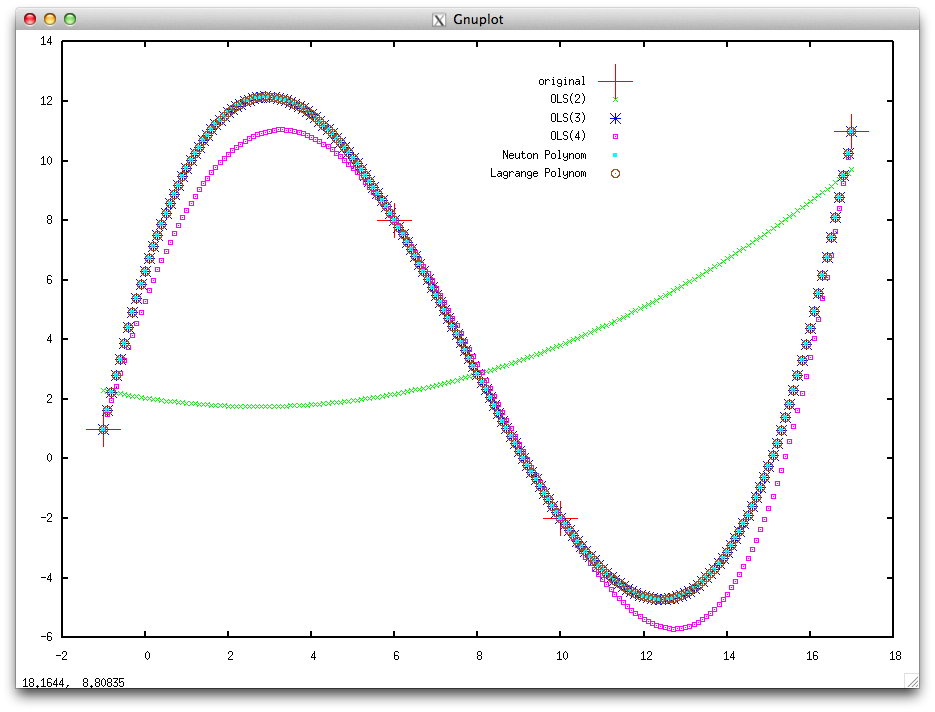
\includegraphics[width=13cm]{interpolations_result.png}
    \caption{Результат работы расчитанных полиномов}
    \label{interpolations_img}
  \end{figure}
  
\newpage
\section{Методы численного интегрирования и дифференцирования}

\subsection{Интегрирование}
Задана функция $f(x) = \frac{x}{sin^2(3x)}$ на интервале $[0.1, 1]$.
Рассчитаем шаг $h$ исходя из условия, что $h = \frac{b-a}{n}$ , где $n=5$ -
количество интервалов, $a$ - нижняя граница интервала, $b$ - верхняя граница
интервала: \\
$h = \frac{1 - 0.1}{5} = 0.18$.

Учитывая полученный шаг, и используя заданную функцию, получим табличные данные: 
\begin{table}[!h]
  \begin{tabular}{|l|l|l|l|l|l|l|}
  \hline
  \bfseries x & 0.1 & 0.28 & 0.46 & 0.64 & 0.82 & 1\\
  \hline
  \bfseries y & 1.14505 & 0.504965 & 0.47716 & 0.724856 & 2.06581 & 50.2138\\
  \hline
  \end{tabular}
\end{table}

\subsubsection{Метод прямоугольников}
Вычислим все $S_{i} = y_{i-1} \cdot h$ где $i = 1..n$. \\
$S_{1} =  1.14505 \cdot 0.18 = 0.206109$ \\
$S_{2} =  0.504965 \cdot 0.18 = 0.0908937$ \\
$S_{3} =  0.47716 \cdot 0.18 = 0.0858888$ \\
$S_{4} =  0.724856 \cdot 0.18 = 0.13047408$\\
$S_{5} =  2.06581 \cdot 0.18 = 0.3718458$\\

Теперь имея набор площадей прямоугольников, можем посчитать значение 
$\int_{0.1}^1 \frac{x}{sin^2(3x)}dx$ зная, что это  $\approx \sum S_{i}$: \\
\begin{displaymath} 
  \sum S_{i} = 0.206109 + 0.0908937 + 0.0858888 + 0.13047408 + 0.3718458 =
  0.88521138
\end{displaymath}

\subsubsection{Метод трапеций}\label{integ_trapezoid}
Вычислим все $S_{i} = (y_{i-1} + y_{i}) \cdot \frac{h}{2}$ где $i = 1..n$. \\
$S_{1} = (1.14505 + 0.504965 ) \cdot 0.09 = 0.14850135$\\
$S_{2} = (0.504965 + 0.47716 ) \cdot 0.09 = 0.08839125$\\
$S_{3} = (0.47716 + 0.724856 ) \cdot 0.09 = 0.10818144$\\
$S_{4} = (0.724856 + 2.06581 ) \cdot 0.09 = 0.25115994$\\
$S_{5} = (2.06581 +  50.2138 )  \cdot 0.09 = 4.7051649$\\

Теперь имея набор площадей трапеций, можем посчитать значение  
$\int_{0.1}^1 \frac{x}{sin^2(3x)}dx$:\\
\begin{displaymath} 
  \sum S_{i} = 0.14850135 + 0.08839125 + 0.10818144 + 0.25115994 + 4.7051649 =
  5.30139888
\end{displaymath}

\subsubsection{Метод Симпсона}
Вычислим все $S_{i} = (y_{i-1} + 4 \cdot y_{i} + y_{i+1}) \cdot \frac{h}{6}$ где
$i = 1..n-1$. \\
$S_{1} = (1.14505 + 4 \cdot 0.504965 + 0.47716) \cdot 0.03 = 0.1092621$\\
$S_{2} = (0.504965 + 4 \cdot 0.47716 + 0.724856) \cdot 0.03 = 0.09415383$\\
$S_{3} = (0.47716 + 4 \cdot 0.724856 + 2.06581) \cdot 0.03 = 0.16327182$\\
$S_{4} = (0.724856 + 4 \cdot 2.06581 + 50.2138) \cdot 0.03 = 1.77605688$\\

Теперь имея набор площадей на интервалах, можем посчитать значение  
$\int_{0.1}^1 \frac{x}{sin^2(3x)}dx$:\\
\begin{displaymath} 
  \sum S_{i} = 0.1092621 + 0.09415383 + 0.16327182 + 1.77605688 = 2.14274463
\end{displaymath}

\subsubsection{Квадратура Гаусса}
Находим значения $t_{i}$ для заданного условием задачи ($[0.1, 1]$) диапазона:

$t_{i} = \frac{b + a}{2} - \frac{b - a}{2} \cdot x_{i}$ , где 
$x = [-\sqrt{\frac{3}{5}}, 0, \sqrt{\frac{3}{5}}]$.\\
$t_{0} = \frac{1 + 0.1}{2} - \frac{1 - 0.1}{2} \cdot \sqrt{\frac{3}{5}}
= 0.20143149895$ \\
$t_{1} = \frac{1 + 0.1}{2} = 0.55$  \\
$t_{2} = \frac{1 + 0.1}{2} + \frac{1 + 0.1}{2} \cdot \sqrt{\frac{3}{5}}
= 0.89856850105$, \\
при этом значения коэффициентов $A_{i}$ соответствуют следующим значениям: \\
$A_{0} = \frac{5}{9} = 0.555555556 $\\
$A_{1} = \frac{8}{9} = 0.888888889 $\\
$A_{2} = \frac{5}{9} = 0.555555556 $\\

Рассчитаем значения функций $y_{i} = f(t_{i})$: \\
$y_{0} = \frac{0.20143149895}{sin^2(3 \cdot 0.20143149895)} = 0.62395456529$\\
$y_{1} = \frac{0.55}{sin^2(3 \cdot 0.55)} = 0.553465$ \\
$y_{2} = \frac{0.89856850105}{sin^2(3 \cdot 0.89856850105)} = 4.831432657 $\\

Зная, что результатом метода квадратуры Гаусса является $\sum A_{i} \cdot
y_{i}$, можем посчитать значение интегрирования: \\

$S = ((0.62395456529 \cdot 0.555555556) 
   + (0.553465 \cdot 0.888888889) 
   + (4.831432657 \cdot 0.555555556)) * 0.45
   = 1.585232
$

\subsubsection{Вычисление интеграла с переменным верхним пределом по методу
трапеций}
В данном задании используется интервал $[a, x]$, где $x \in [a, b]$, с шагом
$h$ (для вычисления значений интеграла на каждом из шагов, будем использовать
полученные результаты из \ref{integ_trapezoid}). 
Необходимо посчитать значения функции $F(x) = \int_{0.1}^x
\frac{x}{sin^2(3x)}dx$. Результатом вычисления является накопленная сумма
площадей и прибавленная к ней площадь добавленного
интервала ($F(x) = S = \sum\limits_{i=1}^k S_i + S_{k+1}$).\\

\begin{enumerate}[label= \arabic{*}:]
  \item 
  $ x = 0.1$ \\
  $a-b = 0.1 - 0.1 = 0$ - поскольку, длинна интервала = 0, то $S_0 = 0$\\
  $S = 0$

  \item 
  $ x = 0.28$ \\ 
  $S = \sum\limits_{i=1}^1 + 0.14850135 = 0 + 0.14850135 = 0.14850135$ \\
  
  \item 
  $ x = 0.46$ \\
  $S = \sum\limits_{i=1}^2 + 0.08839125 = 0.14850135 + 0.08839125 = 0.2368926$\\
  
  \item 
  $ x = 0.64$ \\
  $S = \sum\limits_{i=1}^3 + 0.10818144 = 0.2368926 + 0.10818144 = 0.34507404$\\
  
  \item 
  $ x = 0.82$ \\
  $S = \sum\limits_{i=1}^4 + 0.25115994 = 0.34507404 + 0.25115994 = 0.59623398$\\
  
  \item 
  $ x = 1$ \\
  $S = \sum\limits_{i=1}^5 + 4.7051649 = 0.59623398 + 4.7051649 = 5.30139888$\\
  
\end{enumerate}

\subsubsection{Анализ результатов}
Поскольку шаг был слишком большой,то не удалось получить достаточно корректное
значение интеграла ни одним из методов.

Метод прямоугольников берет на последнем шаге высоту равную значению функции в
предпоследей точке и умножает ее на шаг - получая таким образом прямоугольник
высотой гораздо меньшей чем значение в последней точке. Отсюда берется его
ошибка.

Метод трапеций, напротив, ориентируется на последнюю точку, и захватывает
большую часть площади находящуюся над функцией.

Метод Симпсона показал наилучший результат, поскольку его способ описания прямой
(использованием пораболы) подходит лучше остальных.

\begin{center}
  \begin{tabular}{|l|l|l|l|}
  \hline
  \bfseries М-д прямоугольников & м-д трапеций & м-д Симпсона & квадратура Гаусса\\
  \hline
  \bfseries 0.88521138 & 5.30139888 & 2.14274463 & 1.585232 \\
  \hline
  \end{tabular}
\end{center}

 \begin{figure}[h!]
    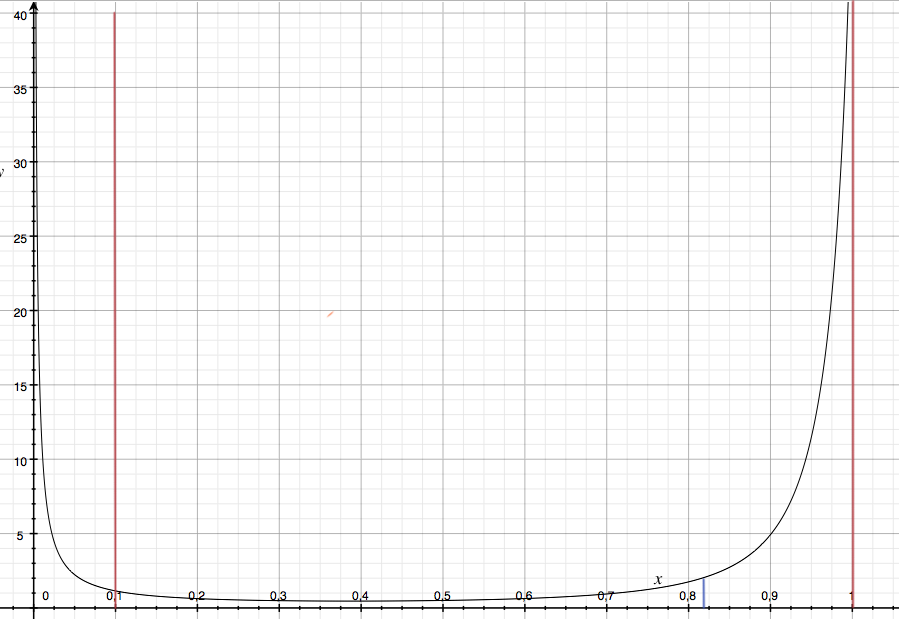
\includegraphics[width=13cm]{result-int.png}
    \caption{Результат работы расчитанных полиномов}
  \end{figure}

\subsection{Дифференцирование}
\subsubsection{Метод центральных разностей}
Зная что $ f'(x) = 
 \frac{dy}{dx} =
 \frac{\Delta y}{\Delta x} =
 \frac{y(x + \Delta x) - y(x - \Delta x)}{2 \Delta x}$, рассчитаем значения
 производной в значениях $x$ указанных в табличных данных для заданий
 интегрирования: \\ 
$f'(x_{0}) = y_{0} = \frac{f(0.1 + 0.18) - f(0.1 - 0.18)}{0.36 } = 5.335$\\
$f'(x_{1})=y_{1} = \frac{f(0.28 + 0.18) - f(0.28 - 0.18)}{0.36 } =
-1.8556$\\
$f'(x_{2})=y_{2} = \frac{f(0.46 + 0.18) - f(0.46 - 0.18)}{0.36 } =
0.6108$\\
$f'(x_{3})=y_{3} = \frac{f(0.64 + 0.18) - f(0.64 - 0.18)}{0.36 } =
4.41292 $\\
$f'(x_{4})y_{4} = \frac{f(0.82 + 0.18) - f(0.82 - 0.18)}{0.36 } =
137.469 $\\
$f'(x_{5})=y_{5} = \frac{f(1 + 0.18) - f(1 - 0.18)}{0.36 } = 16.040$
\subsection{Графическое отображение}
Сводная таблица требуемых данных:
\begin{table}[h!]
  \begin{tabular}{|l|l|l|l|l|l|l|}
  \hline
  \bfseries x & 0.1 & 0.28 & 0.46 & 0.64 & 0.82 & 1\\
  \hline
  \bfseries f(x) & 1.14505 & 0.504965 & 0.47716 & 0.724856 & 2.06581 & 50.2138\\
  \hline
  \bfseries f'(x) & 5.335 & -1.8556 & 0.6108 & 4.41292 & 137.469 & 16.040\\
  \hline
  \bfseries F(x) & 0 & 0.14850135 & 0.2368926 & 0.34507404 & 0.59623398 &5.30139888\\
  \hline
  \end{tabular}
\end{table}

\begin{figure}[h!]
  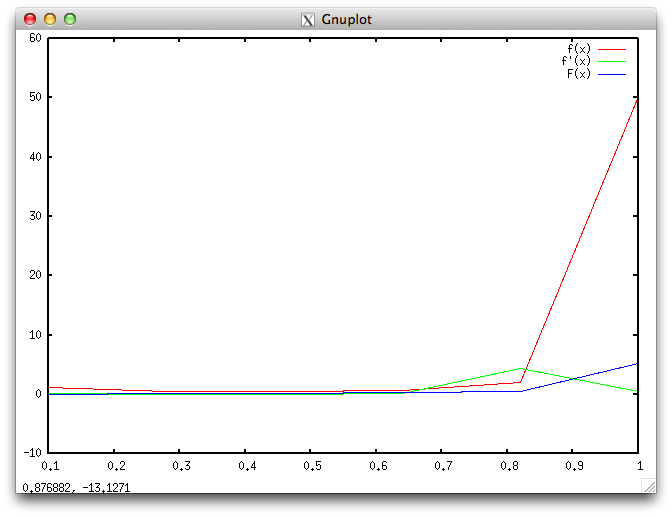
\includegraphics[width=13cm]{result_of_integ_diff.png}
  \caption{Результат вычислений f(x), f'(x) и F(x)}
  \label{interpolations_img}
\end{figure}

\section{Решение нелинейного уравнения}

\begin{displaymath}
  \begin{array}{ccc}
    f(x) = \frac{x}{sin^2(3x)}  \\
    f'(x) = (1 - \frac{6x}{tg(3x)}) \cdot \frac{1}{sin^2(3x)}\\
    f''(x) = \frac{6 \cdot (6x - sin(6x) + 3x \cdot cos(6x))}{sin^4(3x) }\\
  \end{array}
\end{displaymath}

\begin{displaymath}
  \begin{array}{ccc}
    f(x) = N_{g}  \\
    \frac{x}{sin^2(3x)}= 17 \\
    \frac{x}{sin^2(3x)} - 17 = 0 \\
  \end{array}
\end{displaymath}

Точность: $\varepsilon = 0.0001$

Интервал для поиска корней: [0.1; 1]

\subsection{Метод бисекции}
\begin{enumerate}[label= итерация \arabic{*}:]
  \item 
  \begin{math}
    x_{1}=(0.1+1)/2=0.55\\
    a=0.1, b=1\\
    b-a=1-0.1= 0.9\\
    0.9 < \varepsilon \\
    f(a)=-15.854, f(x_{1})= -16.446\\
    f(a) \cdot f(x_{1}) > 0\\
    a=0.55, b=1\\
  \end{math}
  
  \item
  \begin{math}
    x_{2}=(0.55+1)/2=0.775\\
    a=0.55, b=1\\
    b-a=1-0.55= 0.45\\
    0.45 > \varepsilon \\
    f(a)=-16.446, f(x_{2})= -15.540\\
    f(a) \cdot f(x_{2}) > 0 \\
    a=0.775, b=1\\
  \end{math}
  
  \item
  \begin{math}
    x_{3}=(0.775+1)/2=0.8875\\
    a=0.775, b=1\\
    b-a=1-0.775= 0.225\\
    0.225 > \varepsilon \\
    f(a)=-15.540, f(x_{3})= -12.823\\
    f(a) \cdot f(x_{3}) > 0 \\
    a=0.8875, b=1\\
  \end{math}
  
  \item
  \begin{math}
    x_{4}=(0.8875+1)/2=0.94375\\
    a=0.8875, b=1\\
    b-a=1-0.8875= 0.1125\\
    0.1125 > \varepsilon \\
    f(a)=-12.823, f(x_{4})= -6.880\\
    f(a) \cdot f(x_{4}) > 0 \\
    a=0.94375, b=1\\
  \end{math}

  \item 
  \begin{math}
    x_{5}=(0.94375+1)/2=0.971875\\
    a=0.94375, b=1\\
    b-a=1-0.94375= 0.05625\\
    0.05625 > \varepsilon \\
    f(a)=-6.880, f(x_{5})= 2.360\\
    f(a) \cdot f(x_{5}) < 0 \\
    a=0.94375, b=0.971875\\
  \end{math}
  
  \item 
  \begin{math}
    x_{6}=(0.94375+0.971875)/2=0.9578125\\
    a=0.94375, b=0.971875\\
    b-a=0.971875-0.94375= 0.028125\\
    0.028125 > \varepsilon \\
    f(a)=-6.880, f(x_{6})= -3.355\\
    f(a) \cdot f(x_{6}) > 0 \\
    a=0.9578125, b=0.971875\\
  \end{math}

\end{enumerate}

Результат: $x = 0.9578125$.

\subsection{Метод хорд}
Условие сходимости метода: 
\begin{displaymath}
  \begin{array}{ccc}
    f(1) = 33.2137 \\
    f''(1) = 138.576
  \end{array}
\end{displaymath}
- знак не меняется, значит метод применим.\\

\begin{enumerate}[label= итерация \arabic{*}:]
  \item
\begin{math}
  x_{1}=1 - \frac{1-0.1}{33.21376-(-15.8549)} \cdot
  33.2137=0.3908\\
  f(a) = -15.8549, f(x)=-16.5399\\
  f(a) \cdot f(x) >0 \\
  a=0.3908, b=1\\
  |x_{1} - x_{0}| > \varepsilon \\ 
\end{math}

  \item
  \begin{math}
    x_{2}=1 -
    \frac{1-0.3908}{33.2137-(-16.5399)} \cdot
    33.2137=0.5933\\
    f(a) = -16.5399, f(x)=-16.3799\\
    f(a) \cdot f(x) >0 \\
    a=0.5933, b=1\\
    |x_{2} - x_{1}| > \varepsilon \\ 
  \end{math}
   
  \item
\begin{math}
  x_{3}=1 -
  \frac{1-0.5933}{33.2137-(-16.3799)} \cdot 33.2137=0.7276\\
  f(a) = -16.3799, f(x)=-15.9136\\
  f(a) \cdot f(x) >0 \\
  a=0.7276, b=1\\
  |x_{3} - x_{2}| > \varepsilon \\ 
\end{math}
 
  \item 
 \begin{math}
  x_{4}=1 - \frac{1-0.7276}{33.2137-(-15.9136)}
  \cdot 33.2137=0.8158\\
  f(a) = -15.9136, f(x)=-15.0057\\
  f(a) \cdot f(x) >0 \\
  a=0.8158, b=1\\
  |x_{4} - x_{3}| > \varepsilon \\ 
\end{math}

  \item 
\begin{math}
  x_{5}=1 -
  \frac{1-0.8158}{33.2137-(-15.0057)} \cdot 33.2137=0.8731\\
  f(a) = -15.0057, f(x)=-13.4889\\
  f(a) \cdot f(x) >0 \\
  a=0.8731, b=1\\
  |x_{5} - x_{4}| > \varepsilon \\ 
\end{math}
  
  \item 
  \begin{math}
    x_{6}=1 -
    \frac{1-0.8731}{33.2137-(-13.4889)} \cdot
    33.2137=0.9098\\
    f(a) = -13.4889, f(x)=-11.3312\\
    f(a) \cdot f(x) >0 \\
    a=0.9098, b=1\\
    |x_{6} - x_{5}| > \varepsilon \\ 
  \end{math}
\end{enumerate}
Результат: $x = 0.9098$.

\subsection{Метод Ньютона}
$x_{0}=0.55$.
\begin{enumerate}[label= итерация \arabic{*}:]
  \item
  \begin{math}
    x_{0}=0.55\\
    x_{1} = 0.55 - \frac{-16.4465}{1.2698} = 13.5013
  \end{math}
\end{enumerate}
По итогам 1ой итерации видно, что метод вышел за пределы интервала.
Проанализировав функцию, можно сделать вывод, что в необходимый интервал метод не вернется,
поскольку начнет приблежаться к более близким корням относительно вычисленного
значения $x$.

Для того, чтобы метод не выходил из заданного интервала, нужно сжать
начальный интервал так, чтобы начальный $x_0$ был из бассейна Ньютона, который
указывает на корень в необходимом интервале.

Будем искать корень на интервале $[0.5, 1]$.\\
$x_{0}=0.75$.

\begin{enumerate}[label= итерация \arabic{*}:]
\item
\begin{math}
  x_{0} = 0.7500\\
  x_{1} = 0.7500 - \frac{-15.7611}{7.6529} = 2.8095\\
  |2.8095 -0.7500| > \varepsilon\\
\end{math}

\item
\begin{math}
  x_{1} = 2.8095\\
  x_{2} = 2.8095 - \frac{-13.0131}{16.9045} = 3.5793\\
  |3.5793 -2.8095| > \varepsilon\\
\end{math}

\item
\begin{math}
  x_{2} = 3.5793\\
  x_{3} = 3.5793 - \frac{-13.1721}{-4.9833} = 0.9360\\
  |0.9360 -3.5793| > \varepsilon\\
\end{math}

\item
\begin{math}
  x_{3} = 0.9360\\
  x_{4} = 0.9360 - \frac{-8.2663}{160.5773} = 0.9875\\
  |0.9875 -0.9360| > \varepsilon\\
\end{math}

\item
\begin{math}
  x_{4} = 0.9875\\
  x_{5} = 0.9875 - \frac{14.1212}{1063.0069} = 0.9742\\
  |0.9742 -0.9875| > \varepsilon\\
\end{math}

\item
\begin{math}
  x_{5} = 0.9742\\
  x_{6} = 0.9742 - \frac{3.6517}{578.0826} = 0.9679\\
  |0.9679 -0.9742| > \varepsilon\\
\end{math}
\end{enumerate}

Результат: $x = 0.9679$.

\subsubsection{Метод Ньютона: пояснение}
  Метод Ньютона, при начальном $x_{0} = 0.55$ не сходится (см.
  Рис.\ref{equ_newton_img}), поскольку касательная к графику функции при
  $x = 0.55$, `отправляет` значение следующего $x$ далеко от начального
  интервала.
  
  \begin{figure}[h!]
    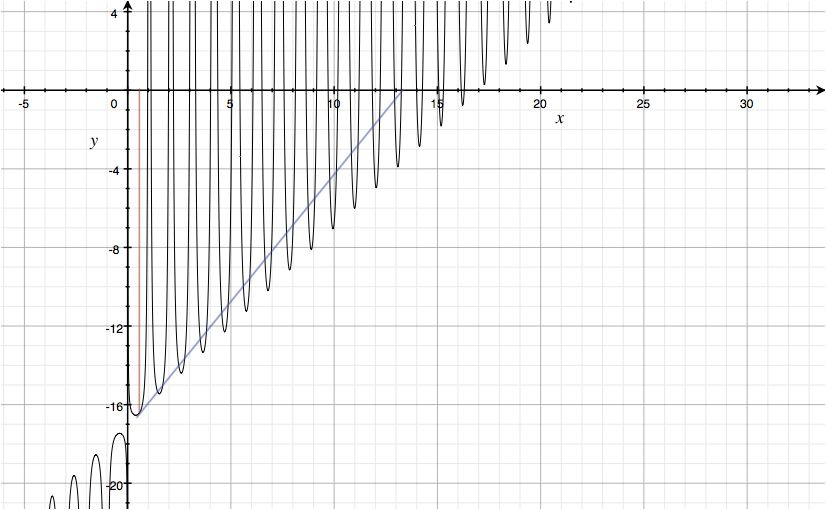
\includegraphics[width=13cm]{equations_newton.png}
    \caption{Первые шаги поиска корня методом Ньютона для функции $x/sin^2(3x)
    - 17$}
    \label{equ_newton_img}
  \end{figure}

\subsection{Метод простых итераций}
Изменим функцию $f(x) = 0$ для использования ее в методе простых итераций:
\begin{enumerate}
  \item домножим правую и левую часть на коррекционный коэффициент
  $k$ -> $k \cdot f(x) = 0$;
  \item вычтим из равенста $x=x$ уравнение $k \cdot f(x) = 0$ и получим
  $x - k \cdot f(x) = x$;
  \item $x$ в правой части уравнения $x$ будем считать за $x_{i+1}$, а $x$ в
  левой части уравнения использовать как $x_i$, $k$ - коррекционный коэффициент и
  равен 0. Назавем вывденную функцию $\psi(x)$.
\end{enumerate} 
Таким образом, была выведена функция для получения следующего значения $x$.

Проверим условие сходимости: $x_0 = 0.55$ подставим в выведенную формулу для
поиска следующего $x$.\\
$x_{1} = x_{0} - 1 \cdot f(x_{0}) = 0.55 - (-16.446)= 16.9965$\\
Подставим $x_{1}$ в $\psi'(x)$, где $\psi'(x) = 1 - f'(x)$ \\
$\psi'(16.9965) = 1.781380$  т.к. вычесленное абсолютное значение больше 1, то
изменим значение коррекционного коэффициента на 0.003. Тогда
$x_{1} = x_{0} - 0.003\cdot f(x_{0}) = 0.55 - 0.003 \cdot (-16.446)= 0.5993$, а
значение $\psi'(0.5993) =0.99421$

\begin{enumerate}[label= итерация \arabic{*}:]
  \item
\begin{math}
  x_{1} = 0.5993\\
  x_{2} = k \cdot f(x_{1}) = 0.5993-0.003 \cdot 0.5993=0.6484\\
  \psi'(x_{2}) = 0.9912\\
  |x_{2} - x_{1}| = |0.6484-0.5993| = 0.0491 > e 
\end{math}

\item
\begin{math}
  x_{2} = 0.6484\\
  x_{3} = k \cdot f(x_{2}) = 0.6484-0.003 \cdot 0.6484=0.6972\\
  \psi'(x_{3}) = 0.9864\\
  |x_{3} - x_{2}| = |0.6972-0.6484| = 0.0488 > e 
\end{math}

\item
\begin{math}
  x_{3} = 0.6972\\
  x_{4} = k \cdot f(x_{3}) = 0.6972-0.003 \cdot 0.6972=0.7454\\
  \psi'(x_{4}) = 0.9781\\
  |x_{4} - x_{3}| = |0.7454-0.6972| = 0.0482 > e 
\end{math}

\item
\begin{math}
  x_{4} = 0.7454\\
  x_{5} = k \cdot f(x_{4}) = 0.7454-0.003 \cdot 0.7454=0.7928\\
  \psi'(x_{5}) = 0.9625\\
  |x_{5} - x_{4}| = |0.7928-0.7454| = 0.0474 > e
\end{math}

\item
\begin{math}
  x_{5} = 0.7928\\
  x_{6} = k \cdot f(x_{5}) = 0.7928-0.003 \cdot 0.7928=0.8388\\
  \psi'(x_{6}) = 0.9301\\
  |x_{6} - x_{5}| = |0.8388-0.7928| = 0.0460 > e 
\end{math}

\item
\begin{math}
  x_{6} = 0.8388\\
  x_{7} = k \cdot f(x_{6}) = 0.8388-0.003 \cdot 0.8388=0.8825\\
  \psi'(x_{7}) = 0.8556\\
  |x_{7} - x_{6}| = |0.8825-0.8388| = 0.0437 > e 
\end{math}

\end{enumerate}
Результат: $x = 0.8825$.

\subsection{Результат}
В таблице приведены результаты, которых достигли методы за 6 итераций.
\begin{center}
  \begin{tabular}{|l|l|l|l|}
  \hline
  \bfseries М-д бисекции & м-д хорд & м-д Ньютона & м-д простых итераций\\
  \hline
  \bfseries 0.9578125 & 0.9098 & 0.9679 & 0.8825 \\
  \hline
  \end{tabular}
\end{center}

\section{Решение линейного дифференциального уравнения 2-го порядка}
Общее задание вида $y''(t) + 5\cdot y'(t) + N_s \cdot y(t) = N_g$ принимает вид
$y''(t) + 5\cdot y'(t) + 16 \cdot y(t) = 17$, а начальные ограничения 
$y(0) = 5, y'(0) =10$. \\
Рассчитаем шаг $h$: \\
\begin{enumerate}
  \item Решим характерестическое уравнение $a^2 + 5a + 16 = 17$:\\
  привидем уравнение к однородному виду $a^2 + 5a -1 =0$;\\
  вычислим дискриминант $D = b^2-4ac = 25 -4*1*(-1) = 29$;\\
  найдем корни: 
  \begin{itemize}
    \item $x_1 = \frac{-b + \sqrt{D}}{2a} = \frac{-5 + \sqrt{29}}{2} = 0.19$
    \item $x_2 = \frac{-b - \sqrt{D}}{2a} = \frac{-5 - \sqrt{29}}{2} = -5.19$
  \end{itemize}
  
  \item $min: \{|0.19|, |-5.19| \} = 0.19$
  
  \item $\tau = 1/0.19 = 5.263$
   
  \item $T = \frac{3}{4} \cdot \tau = \frac{3}{4} \cdot 5.263 = 3.95$
  
  \item $h = \frac{T}{20} = \frac{3.95}{20} = 0.1975$
  
\end{enumerate}

Привидем задачу к виду задачи Коши:
\begin{math}
\left\{ 
\begin{array}{cc}
  y' = z,             & y(0) = 5 \\ 
  z' = 17 - 5z - 16y, & y'(0) = 10
\end{array}
\right\}
\end{math}

\subsection{Метод Рунге-Кутта 4-ого порядка}
\begin{math}
  y_{i+1} = y_i + \frac{h}{6} (k_0 + 2k_1 + 2k_2 + k_3)\\
  z_{i+1} = z_i + \frac{h}{6} (l_0 + 2l_1 + 2l_2 + l_3)
\end{math} 
\\
\begin{math}
\begin{array}{rl}
  k_0 = z_i,                  & l_0 = 17 - 5z_i - 16y_i \\ 
  k_1 = z_i + \frac{hl_0}{2}, & l_1 = 17 - 5\frac{z_i + hl_0}{2} - 16\frac{y_i +  hk_0}{2} \\
  k_2 = z_i + \frac{hl_1}{2}, & l_2 = 17 - 5\frac{z_i + hl_1}{2} - 16\frac{y_i +  hk_1}{2} \\
  k_3 = z_i + hl_2,           & l_3 = 17 - 5(z_i + hl_2) - 16(y_i + hk_2)\\
\end{array}
\end{math} \\
Поскольку, для поиска графика функции необходимо сделать 20 итераций в каждой из
которых по 10 вычислений, то отобразим лишь вычисления для первой итерации.
\begin{itemize}
  \item $k_0 = z_i = 10$
  \item $l_0 = 17 - 5z_i - 16y_i  
  = 17 - 5 \cdot 10 - 16 \cdot 5 
  = -113$
  \item $k_1 = z_i + \frac{hl_0}{2} 
  = 10 + \frac{0.1975 \cdot (-113)}{2}
  =-1.15875$
  \item $l_1 = 17 - 5\frac{z_i + hl_0}{2} - 16\frac{y_i +  hk_0}{2}
  = 17 - 5\frac{10 + 0.1975\cdot (-113)}{2} - 16\frac{5 +  0.1975\cdot 10}{2} 
  = -48.00625$
  \item $k_2 = z_i + \frac{hl_1}{2} 
  = 10 + \frac{0.1975 \cdot (-48.00625)}{2} 
  = 5.2593828125$
  \item $l_2 = 17 - 5\frac{z_i + hl_1}{2} - 16\frac{y_i +  hk_1}{2} 
  = 17 - 5\frac{10 + 0.1975 \cdot (-48.00625)}{2} - 16\frac{5 +  0.1975 \cdot(-1.15875)}{2} 
  = -62.4660890625$
  \item $k_3 = z_i + hl_2 
  = 10 + 0.1975 \cdot (-62.4660890625) 
  = -2.3370$
  \item $l_3 = 17 - 5(z_i + hl_2) - 16(y_i + hk_2) 
  = 17 - 5(10 + 0.1975 \cdot (-62.4660890625)) - 16(5 + 0.1975 \cdot 5.2593828125) 
  = -67.93438$
  
  \item $y_{i+1} = y_i + \frac{h}{6} (k_0 + 2k_1 + 2k_2 + k_3)
  = 5 + \frac{ 0.1975}{6} (10 + 2\cdot (-1.15875) + 2\cdot (5.2593828125)  +(-2.3370)) 
  = 5.52219$
\end{itemize}

Далее для вычислений была использована программа реализующая метод Рунге-Кутта
(код см. в \ref{rungekuttaalg}).

\begin{figure}[h!]
  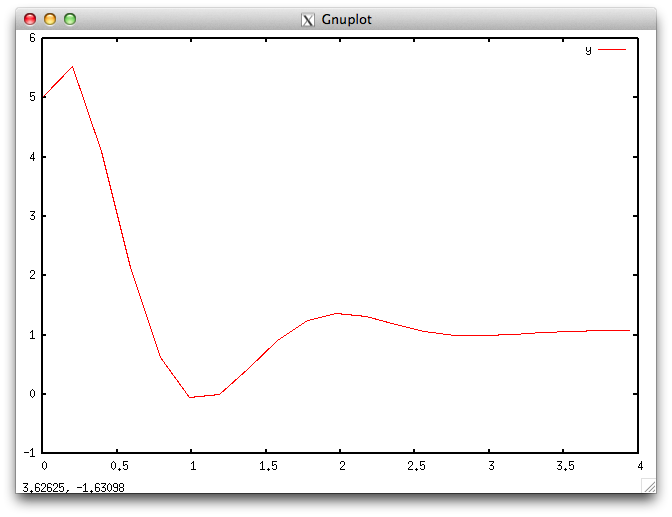
\includegraphics[width=13cm]{rungekutt.png}
  \caption{Результат вычислений произведенных методом Рунге-Кутта}
\end{figure}

\subsubsection{Програмный код для метода Рунге-Кутта}\label{rungekuttaalg}
\begin{lstlisting}
var h = 0.1975

function countParams(cur) {
  kls = {}
  kls.k0 = cur.z
  kls.l0 = 17 - 5*cur.z - 16 *cur.y
  kls.l1 = 17 - 5*((cur.z + h* kls.l0)/2) - 16 *(cur.y + (h*kls.k0)/2)
  kls.k1 = cur.z + (h*kls.l0)/2

  kls.l2 = 17 - 5*((cur.z + h* kls.l1)/2) - 16 *(cur.y + (h*kls.k1)/2)
  kls.k2 = cur.z + (h*kls.l1)/2

  kls.l3 = 17 - 5*((cur.z + h* kls.l2)) - 16 *(cur.y + (h*kls.k2))
  kls.k3 = cur.z + (h*kls.l2)
  return kls
} 

function nextCurZY(cur, h, kls){
  var nextCur = {
      y: cur.y + h/6*(kls.k0 + 2* kls.k1 + 2*kls.k2 + kls.k3),
      z: cur.z + h/6*(kls.l0 + 2* kls.l1 + 2*kls.l2 + kls.l3)
  }
  return nextCur
}

var cur = {
  y: 5,
  z: 10
}

for(var i=0; i < 3.95; i+=h) {
  var kls = countParams(cur)
  cur = nextCurZY(cur, h, kls)
}
\end{lstlisting}

\section{MATLAB}
\subsection{Решение ОДУ}
Задание:
\begin{math}
\left\{ 
\begin{array}{l}
  x' = x \cdot y - a_1 \cdot x, \\
  y' = b_1 \cdot x \cdot y - b_2  \cdot y^2 - b_3  \cdot y - b_4 \cdot (x-z),\\ 
  z' = c_1 -c_2  \cdot x.\\
\end{array}
\right\}
\end{math}\\
при $a_1 = 0.21, b_1=0.15, b_2 = 0.06, b_3 = 0.08, b_4 = 0.1, c_1 = 0.01,
c2=0.03$, и начальных условиях $x(0) = 1, y(0) = 0.1, z(0) = 0.75$.

Необходимо отобразить: 
\begin{itemize}
  \item x(t) - валовой продукт;
  \item y(t) - темп роста валового продукта;
  \item z(t) - платежеспособный спрос;
  \item фазовый портрет.
\end{itemize}

Вычисления производить на интервале $[0; 100]$.
\subsubsection{Выполнение}
\begin{itemize}
  \item m-file
  \begin{lstlisting}
  function res = getXYZ(time, xyz)
    x = xyz(1);
    y = xyz(2);
    z = xyz(3);
    
    koeffs = [0.21, 0.15, 0.06, 0.08, 0.1, 0.01, 0.03];
    a1 = koeffs(1);
    b1 = koeffs(2);
    b2 = koeffs(3);
    b3 = koeffs(4);
    b4 = koeffs(5);
    c1 = koeffs(6);
    c2 = koeffs(7);
    
    dx = x*y - a1*x;
    dy = b1*x*y - b2*y^2 - b3*y - b4*(x-z);
    dz = c1 - c2*x;

    res = [dx; dy; dz];
  end
  \end{lstlisting}
  \item command-line
  \begin{lstlisting}
  >> initXYZ = [1, 0.1, 0.75];
  >> [time, xyz] = ode45('getXYZ', [0,100], initXYZ);
  >> figure (1), plot(time, xyz), grid on;
  >> figure (2), comet3(xyz(:,1), xyz(:,2), xyz(:,3));
  \end{lstlisting}
\end{itemize}

\begin{figure}
  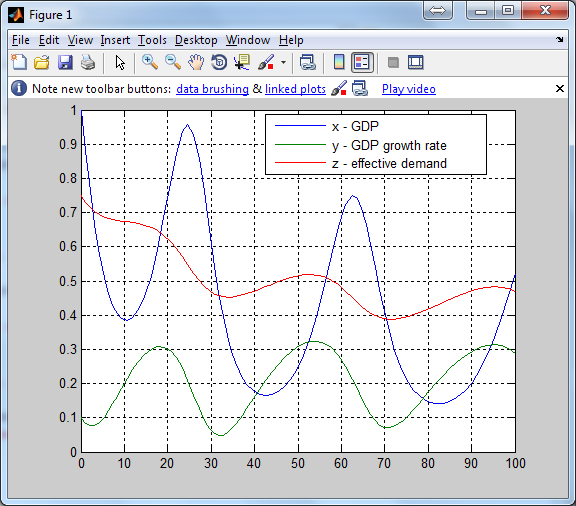
\includegraphics[width=13cm]{matlab24-1.png}
  \caption{x(t) - валовой продукт; y(t) - темп роста валового продукта; z(t) -
  платежеспособный спрос;}
\end{figure}

\begin{figure}
  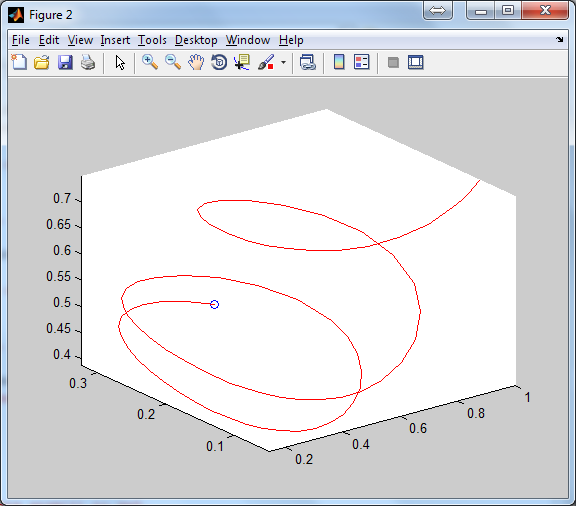
\includegraphics[width=13cm]{matlab24-2.png}
  \caption{Фазовый портрет}
\end{figure}
 
 \newpage
\subsection{Минимизация функций}
\begin{math}
\begin{array}{l}
  f(x1, x2) = e^{x_1^2 + 5x_2^2} + x_1^2 - 80 x_2^2\\
  x_1 + 2x_2^2 \leq 1;\\
  x_1^2 + x_2^2 - 4x_1 \leq 0;\\
  x_1^2 + x_2^2 - x_1 - x_2 \leq 0;\\
\end{array}
\end{math}\\
Минимизировать функцию $f(x1, x2)$ при начальных учловиях $x_1 = 1, x_2 = 1$.
\subsubsection{Выполнение}
\begin{itemize}
  \item fun.m file
  \begin{lstlisting}
  function f = fun(x)
    f = exp((x(1)^2) + 5*(x(2)^2)) + (x(1)^2) - 80 * (x(2)^2);
  end
  \end{lstlisting}
  
  \item mycon.m file
  \begin{lstlisting}
  function [ g, ce ] = mycon( x )
    g(1) = x(1) + 2*power(x(2),2) -1;
    g(2) = power(x(1),2) + power(x(2),2) - 4*x(1);
    g(3) = power(x(1),2) + power(x(2),2) - x(1) - x(2);
    ce=[];
  end
  \end{lstlisting}
  
  \item command-line
  \begin{lstlisting}
    >> x = fmincon ('fun', x0, [],[],[],[],[],[], 'mycon')
    x = 0.4469   -0.2051
    >> fun(x)
    ans = -1.6590
  \end{lstlisting}
\end{itemize}
Минимальное значение функции $f$ достигается при входных данных 
$x_1 = 0.4469, x_2 = -0.2051$ и достигает при этом значения $-1.6590$. 
\end{document}
